
\chapter{Lunedì 22/03/2021}
\section{Corrispondenza C++-Assembler: classi}
\begin{verbatim}
	class c {
		int i;
		long j;
		....
		c();
		c(int);
		~c();
	};
\end{verbatim}
Parliamo di classi: esse permettono di raggruppare insieme dati e codice, definire un nuovo tipo (astratto) e la sua rappresentazione interna (sottotipi), definire quali operazioni è possibile eseguire su questo sottotipo.
Possiamo definire \emph{funzioni membro}, distinguere la visibilità dei vari elementi definiti in una classe, definire funzioni particolari come costruttori (anche più di uno in base ai tipi) e i distruttori.
\subsection{Prima implementazione (da C++ a C): compilatore \emph{cfront}} La prima implementazione è avvenuta con un compilatore chiamato \emph{cfront} in cui si passa da C++ a C. Il linguaggio verso cui si traduce non deve essere per forza a basso livello.
\paragraph{Come traduciamo una chiamata di funzione membro?} Prendiamo il seguente codice
\begin{verbatim}
	int main() {
		c miac;
		miac.f(...);
	}
\end{verbatim}
\begin{itemize}
	\item Il compilatore osserva la definizione della classe: questa non produce di per se alcun codice, ma determina una struttura dati interna al compilatore. Il compilatore saprà che esiste una struttura dati che presenta certi dati e certe funzioni membro, con costruttore e distruttore.
	\item Quando vede dichiarata un'istanza di quell'oggetto il compilatore si preoccupa di allocare spazio per quell'istanza.
	\item Quando vede un'invocazione della funzione membro di un oggetto verifica che la si possa chiamare in quel punto (elemento public o no?). Solo dopo questo step traduce la chiamata.
\end{itemize}

\paragraph{Allocazione dell'oggetto} Lo spazio allocato per l'oggetto è lo spazio delle sue variabili membro. La sua parte dati viene tradotta in uno struct:
\begin{verbatim}
	struct c {
		int i;
		long j;
	};
\end{verbatim}
Le funzioni membro diventano funzioni globali, definite però all'interno di una classe. I nomi non coincideranno con quelli delle funzioni: due funzioni globali non possono avere stesso nome, significherebbe impedire a due classi diverse di assumere lo stesso nome per una funzione membro.
\paragraph{Argomento implicito nelle funzioni} Le funzioni membro ricevono, in modo implicito, un puntatore all'oggetto su cui devono lavorare
\begin{verbatim}
	void c_f(c* this, ...)
\end{verbatim}
\paragraph{Dereferenziazione} Sappiamo che scrivendo una cosa del genere
\begin{verbatim}
	void c_f(c* this, ...) {
		i = 10;
	}
\end{verbatim}
il compilatore intenderà i come il campo dell'oggetto su cui la funzione membro è stata chiamata. 
\begin{verbatim}
	void c_f(c* this, ...) {
		this->i = 10;
	}
\end{verbatim}
Abbiamo una dereferenziazione implicita (nulla di nuovo rispetto a quanto visto a Fondamenti di programmazione). Segue una traduzione del main di questo tipo
\begin{verbatim}
	int main() {
		c miac;
		c_f(&miac, ...);
	}
\end{verbatim}
\clearpage

\subsection{Implementazione attuale (da C++ ad Assembler direttamente)}
Adesso \emph{cfront} non viene più utilizzato. Abbiamo compilatori che effettuano un passaggio diretto da C++ ad Assembler. Non si hanno grandi differenze concettuali rispetto al \emph{cfront}. 
\paragraph{Cosa dobbiamo sapere?}
\begin{itemize}
	\item Le regole per la traduzione dei nomi delle funzioni membro.
	\item Come viene passato il puntatore \emph{this}.
\end{itemize}

\subsubsection{Traduzione dei nomi delle funzioni membro}
\begin{verbatim}
	class c {
		tipoR funz(tipo1, ..., tipoN)
	}
\end{verbatim}
Il nome della funzione viene tradotto in Assembler nello stesso modo in cui faceva \emph{cfront}. In particolare, il nome della funzione deve contenere il nome della classe. Vediamo le regole:
\begin{itemize}
	\item Si parte con
	\begin{verbatim}
		_Z
	\end{verbatim}
	\item Tutti i caratteri che servono a definire di quale funzione membro stiamo parlando sono posti tra due lettere: N ed E
	\begin{verbatim}
		_ZN    ...       E
	\end{verbatim}
	Indichiamo il nome della classe e il nome della funzione negli stessi modi visti nella scorsa lezione
	\begin{verbatim}
		_ZN1c4funzE
	\end{verbatim}
	Prima il nome della classe, dopo il nome della funzione
	\item Segue la traduzione dei tipi della funzione con i modi già visti, \textbf{SENZA} contare il parametro implicito \emph{this}. Unica differenza: se uno di questi tipi si rifà alla classe associata alla funzione membro il nome della classe non viene ripetuto, ma si pone
	\begin{verbatim}
		S_
	\end{verbatim}
\end{itemize}
\paragraph{Esempio} Vediamo un esempio con la seguente classe
\begin{verbatim}
	class miac {
		void funz1(); <---- _ZN4miac5funzEv
		void funz2(int); <---- _ZN4miac5funzEi
		void funz2(miac*) <---- _ZN4miac5funzEPS_
	}
\end{verbatim}
La regola è un po' più complicata ma ci limiteremo a questo. Il compilatore cerca di ridurre al minimo le ridondanze, per evitare problemi relativi alla lunghezza delle stringhe nel collegatore.
\paragraph{Costruttori} I costruttori si indicano col seguente nome
\begin{verbatim}
	C1
\end{verbatim}
La cosa non è fonte di equivoci: tutti i nomi definiti da un utente iniziano sempre con un numero.
\paragraph{Distruttori} I distruttori si indicano in modo simile
\begin{verbatim}
	D1
\end{verbatim}

\section{Esercizio dalle diapositive di Frosini}
\begingroup
\small
\subsection{Primo esercizio}
\begin{framed}
	\noindent \textbf{Codice C++}
	\begin{verbatim}
		// programma classe1, file clai1.cpp
	\end{verbatim}
	\begin{multicols}{2}
		\begin{verbatim}
			#include "servi.cpp"
			class clai { 
				int ix, iy, iz;
				public:
				clai();
				clai(int, int, int);
				// ...
				void stampa();
				clai somma(int, int, int);
			};
			
			clai::clai() { 
				ix = 0; iy = 0; iz = 0;
			}
			
			clai::clai(int a, int b, int c) { 
				ix = a; iy = b; iz = c;
			}
			
			
			void clai::stampa() { 
				scriviint(ix); 
				scriviint(iy); 
				scriviint(iz);
				nuovalinea();
			}
			
			clai clai::somma(int a, int b, int c) { 
				clai temp;
				temp.ix = ix+a;
				temp.iy = iy+b;
				temp.iz = iz+c;
				
				return temp;
			}
		\end{verbatim}
	\end{multicols}
\end{framed}
\paragraph{Traduzione di \emph{stampa}} 
\begin{verbatim}
	.global  _ZN4clai6stampaEv
	_ZN4clai6stampaEv:
	push %rbp
	mov %rsp, %rbp
	sub $16, %rip
	mov %rdi, -8(%rbp)
	
	mov -8(%rbp), %rax # this
	mov (%rax), %edi # this->ix
	call scriviint
	
	mov -8(%rbp), %rax # this
	mov 4(%rax), %edi # this->iy
	call scriviint
	
	mov -8(%rbp), %rax # this
	mov 8(%rax), %edi # this->iz
	call scriviint
	
	call nuovalinea # Non ho argomenti in ingresso
	
	leave
	ret
\end{verbatim}

\begin{itemize}
	\item \emph{stampa} è una funzione globale che ha in ingresso un solo parametro, quello implicito \emph{this}.
	\item Scriviamo il nome della funzione
	\begin{verbatim}
		_ZN4clai6stampaEv
	\end{verbatim}
	\begin{itemize}
		\item Inizio con i soliti caratteri: \emph{$\_$Z}.
		\item Abbiamo una funzione membro, dunque poniamo nome della classe e nome della funzione membro tra le lettere \emph{N} ed \emph{E}.
		\item Concludo con la lettera \emph{v} (la funzione non presenta parametri in ingresso, \emph{this} non si considera)
	\end{itemize}
	\item Per quanto riguarda il record di attivazione nulla di strano (l'unico elemento da considerare è il parametro \emph{this})
	\begin{center}
		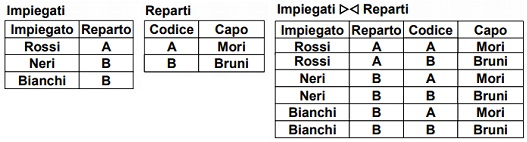
\includegraphics{img/39.PNG}
	\end{center}  
	solito prologo
	\begin{verbatim}
		push %rbp
		mov %rsp, %rbp
		sub $16, %rip
		mov %rdi, -8(%rbp)
	\end{verbatim}
	\item La funzione si limita semplicemente a chiamare quattro funzioni esterne alla classe. I valori posti come parametri di queste funzioni sono sempre dati membro dell'istanza della classe. Segue che dovrò usare il puntatore this per recuperare questi dati, mediante indirizzamento indiretto. 
	\begin{verbatim}
		mov -8(%rbp), %rax # this
		mov (%rax), %edi # this->ix
		call scriviint
		
		mov -8(%rbp), %rax # this
		mov 4(%rax), %edi # this->iy
		call scriviint
		
		mov -8(%rbp), %rax # this
		mov 8(%rax), %edi # this->iz
		call scriviint
		
		call nuovalinea # Non ho argomenti in ingresso
	\end{verbatim}
	\item Concludiamo allo stesso modo con \emph{leave} e \emph{ret}.
\end{itemize}
\paragraph{Traduzione dei costruttori}
I costruttori hanno una sintassi particolare, non restituiscono niente all'apparenza (lo standard suggerisce che siano void). Si adotta una convenzione: la restituzione dell'indirizzo dell'oggetto costruito.
\begin{multicols}{2}
	\begin{verbatim}
		.global _ZN4claiC1Eiii
		_ZN4claiC1Eiii: 
		push %rbp
		mov %rsp, %rbp
		sub $32, %rip
		
		mov %rdi, -8(%rbp)
		# mov %esi, -24(%rbp)
		# mov %edx, -28(%rbp)
		# mov %ecx, -16(%rbp)
		
		mov %esi, (%rdi)
		mov %edx, 4(%rdi)
		mov %ecx, 8(%rdi)
		
		mov %rdi, %rax
		leave
		ret
	\end{verbatim}
	\columnbreak
	\begin{verbatim} 
		.global _ZN4claiC1Ev
		_ZN4claiC1Ev:
		push %rbp
		mov %rsp, %rbp
		sub $16, %rip
		mov %rdi, -8(%rbp)
		
		movl $0, (%rdi)  # this->ix = 0
		movl $0, 4(%rdi)  # this->iy = 0
		movl $0, 8(%rdi)  # this->iz = 0
		
		mov %rdi, %rax
		leave
		ret
	\end{verbatim}
\end{multicols}
\begin{itemize}
	\item \textbf{Primo costruttore (quello senza argomenti)}:
	\begin{itemize}
		\item Scriviamo il nome della funzione
		\begin{verbatim}
			_ZN4claiC1Ev
		\end{verbatim}
		\item Solito prologo per il record di attivazione (stessa struttura vista per la funzione \emph{stampa})
		\begin{verbatim}
			push %rbp
			mov %rsp, %rbp
			sub $16, %rip
			mov %rdi, -8(%rbp)
		\end{verbatim}
		\item Poniamo tutte le variabili della classe uguali a zero, usando un indirizzamento indiretto con displacement
		\begin{verbatim}
			movl $0, (%rdi)  # this->ix = 0
			movl $0, 4(%rdi)  # this->iy = 0
			movl $0, 8(%rdi)  # this->iz = 0
		\end{verbatim}
		\item Restituiamo l'indirizzo dell'oggetto costituito
		\begin{verbatim}
			mov %rdi, %rax
		\end{verbatim}
		\item Concludiamo allo stesso modo
		\begin{verbatim}
			leave
			ret
		\end{verbatim}
	\end{itemize}
	\item \textbf{Secondo costruttore (quello con argomenti)}:
	\begin{itemize}
		\item Scriviamo il nome della funzione
		\begin{verbatim}
			_ZN4claiC1Eiii
		\end{verbatim}
		\item Il record di attivazione conterrà al suo interno anche i parametri in ingresso \emph{a}, \emph{b}, \emph{c}.
		\begin{center}
			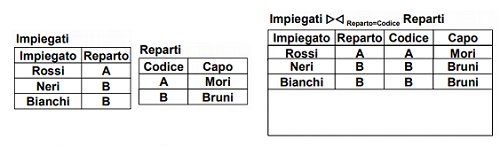
\includegraphics{img/40.PNG}
		\end{center}  
		scriviamo il prologo
		\begin{verbatim}
			push %rbp
			mov %rsp, %rbp
			sub $32, %rip
			
			mov %rdi, -8(%rbp)
			mov %esi, -24(%rbp)
			mov %edx, -28(%rbp)
			mov %ecx, -16(%rbp)
		\end{verbatim}
		in aggiunta ad rdi spostiamo anche il contenuto dei parametri in ingresso. 
		\item Aggiorniamo i valori delle variabili. Facciamo la cosa velocemente, passando direttamente i valori dai registri
		\begin{verbatim}
			mov %esi, (%rdi)
			mov %edx, 4(%rdi)
			mov %ecx, 8(%rdi)
		\end{verbatim}
		chiaramente il compilatore, se chiediamo ottimizzazione, farà così e non allocherà quanto allocato prima nel record di attivazione.
		\item Restituiamo l'indirizzo dell'oggetto costituito
		\begin{verbatim}
			mov %rdi, %rax
		\end{verbatim}
		\item Concludiamo allo stesso modo
		\begin{verbatim}
			leave
			ret
		\end{verbatim}
	\end{itemize}
\end{itemize}
\paragraph{Traduzione della funzione \emph{somma}} La funzione somma presenta al suo interno un'istanza temporanea della classe, e la restituisce!
\begin{verbatim}
	.global _ZN4clai5sommaEiii
	_ZN4clai5sommaEiii:
	push %rbp
	mov %rsp, %rbp
	sub $48, %rsp
	
	mov %rdi, -8(%rbp)
	mov %esi, -24(%rbp)
	mov %edx, -28(%rbp)
	mov %ecx, -16(%rbp)
	
	lea -40(%rbp), %rdi
	call _ZN4claiC1Ev
	
	mov -8(%rbp), %rdi # sposto l'indirizzo dell'oggetto temp in rdi
	
	mov -24(%rbp), %eax 
	add (%rdi), %eax 
	mov %eax, -40(%rbp)
	
	mov -20(%rbp), %eax
	add 4(%rdi), %eax 
	mov %eax, -36(%rbp) 
	
	mov -16(%rbp), %eax 
	add 8(%rdi), %eax 
	mov %eax, -32(%rbp) 
	
	mov -40(%rbp), %rax
	mov -32(%rbp), %edx
	
	leave
	ret
\end{verbatim}
\begin{itemize}
	\item Scriviamo il nome della funzione
	\begin{verbatim}
		_ZN4clai5sommaEiii
	\end{verbatim}
	\item Il record di attivazione includerà le variabili relative all'istanza \emph{temp}
	\begin{center}
		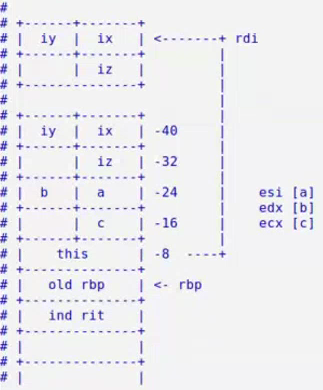
\includegraphics{img/41.PNG}
	\end{center}  
	Abbiamo incluso anche i parametri, nonostante non sia cosa necessaria. Poniamo in memoria i parametri passati mediante registri
	\begin{verbatim}
		mov %rdi, -8(%rbp)
		mov %esi, -24(%rbp)
		mov %edx, -28(%rbp)
		mov %ecx, -16(%rbp)
	\end{verbatim}
	\item La creazione di un'istanza \emph{temp} non si traduce in una semplice allocazione di spazio: dobbiamo creare l'oggetto, cioè chiamare il costruttore!
	\begin{verbatim}
		lea -40(%rbp), %rdi
		call _ZN4claiC1Ev
	\end{verbatim}
	il compilatore ottiene l'etichetta partendo dalla dichiarazione (non dalla definizione).
	\item Eseguiamo le addizioni
	\begin{verbatim}
		mov -8(%rbp), %rdi # sposto l'indirizzo dell'oggetto temp in rdi
		
		mov -24(%rbp), %eax 
		add (%rdi), %eax 
		mov %eax, -40(%rbp)
		
		mov -20(%rbp), %eax
		add 4(%rdi), %eax 
		mov %eax, -36(%rbp) 
		
		mov -16(%rbp), %eax 
		add 8(%rdi), %eax 
		mov %eax, -32(%rbp) 
	\end{verbatim}
	\item Dobbiamo restituire l'oggetto, ma non possiamo limitarci a passare a un indirizzo. In questo momento l'istanza \emph{temp} è allocata nel record di attivazione, dobbiamo renderla disponibile. Quello che dobbiamo fare in teoria è chiamare il \emph{costruttore di copia}. In questo caso non lo abbiamo, quindi ci limitiamo a restituire l'oggetto temporaneo copiandolo nei registri (è un caso particolare, si traduce il tutto nel ritorno di una struttura)
	\begin{verbatim}
		mov -40(%rbp), %rax
		mov -32(%rbp), %edx
	\end{verbatim}
	\item Dopo aver fatto ciò dovrei chiamare il distruttore di \emph{clai} per l'istanza \emph{temp}. Non esiste un distruttore, quindi non abbiamo da fare altro.
	\item Concludiamo allo stesso modo
	\begin{verbatim}
		leave
		ret
	\end{verbatim}
\end{itemize}

\subsection{Secondo esercizio}
\begin{framed}
	\noindent \textbf{Codice C++}
	\begin{verbatim}
		// programma classe2, file main2.cpp
	\end{verbatim}
	\begin{multicols}{2}
		\begin{verbatim}
			class clai { 
				int ix, iy, iz;
				public:
				clai();
				clai(int, int, int);
				clai somma(int, int, int);
				void stampa();
			};
		\end{verbatim}
		\columnbreak
		\begin{verbatim}
			int main() { 
				clai c1, c2(1, 2, 3), c3;
				c1 = c2.somma(5, 10, 15); 
			}
		\end{verbatim}
	\end{multicols}
\end{framed}
\begin{multicols}{2}
	\paragraph{Traduzione del main}
	\begin{verbatim}
		.global main
		main:
		push %rbp
		mov %rsp, %rbp
		sub $48, %rsp
		
		lea -12(%rbp), %rdi
		call _ZN4claiC1Ev
		
		lea -24(%rbp), %rdi
		mov $1, %esi
		mov $2, %edx
		mov $3, %ecx
		call _ZN4claiC1Eiii
		
		lea -36(%rbp), %rdi
		call _ZN4claiC1Ev
		
		lea -24(%rbp), %rdi
		mov $5, %esi
		mov $10, %edx
		mov $15, %ecx
		call _ZN4clai5sommaEiii
		
		mov %rax, -12(%rbp)
		mov %edx, -4(%rbp)
		
		leave
		ret
	\end{verbatim}
\end{multicols}
\begin{itemize}
	\item La parte relativa alla classe non genera codice Assembler: ciò avviene col main, con le definizioni di istanze e le chiamate di funzioni.
	\item Nella struttura del record di attivazione giochiamo a \emph{Tetris}
	\begin{center}
		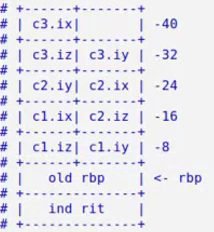
\includegraphics[scale=.9]{img/42.PNG}
	\end{center}  
	solito prologo dove riserviamo una parte della pila
	\begin{verbatim}
		push %rbp
		mov %rsp, %rbp
		sub $48, %rsp
	\end{verbatim}
	\item Inizializziamo le istanze \emph{c1}, \emph{c2} e \emph{c3} della classe \emph{clai}
	\begin{verbatim}
		lea -12(%rbp), %rdi # pongo l'argomento implicito this
		call _ZN4claiC1Ev # Chiamo il costruttore default
		
		lea -24(%rbp), %rdi # Argomento implicito this
		mov $1, %esi   # Primo argomento esplicito
		mov $2, %edx  # Secondo argomento esplicito
		mov $3, %ecx   # Terzo argomento esplicito
		call _ZN4claiC1Eiii # Chiamo il costruttore con tre argomenti int
		
		lea -36(%rbp), %rdi # pongo l'argomento implicito this
		call _ZN4claiC1Ev # Chiamo il costruttore default
	\end{verbatim}
	\item Traduciamo l'operazione di assegnamento
	\begin{verbatim}
		lea -24(%rbp), %rdi # Argomento implicito this
		mov $5, %esi # Primo argomento esplicito
		mov $10, %edx # Secondo argomento esplicito
		mov $15, %ecx # Terzo argomento esplicito
		call _ZN4clai5sommaEiii # Chiamata della funzione c2.somma(int, int, int)
		
		# assegnamento del contenuto restituito dalla funzione membro c2.somma a c1
		mov %rax, -12(%rbp) 
		mov %edx, -4(%rbp)
	\end{verbatim}
	Ricordiamo che abbiamo un caso particolare che ci permette di restituire l'istanza \emph{temp} come una struttura.
	\item Concludiamo allo stesso modo
	\begin{verbatim}
		leave
		ret
	\end{verbatim}
\end{itemize}
\endgroup